\documentclass{beamer}
\usepackage[utf8]{inputenc}
\usepackage{graphicx}

\hypersetup{
    colorlinks,%
    citecolor=blue,%
    filecolor=blue,%
    linkcolor=blue,%
    urlcolor=blue 
    %urlcolor=mygreylink     % can put red here to better visualize the links
}

\author[Sowmya Vajjala]{Instructor: Sowmya Vajjala}

\title[LING 520]{LING 520: Computational Analysis of English}
\subtitle{Semester: FALL '16}

\date{8 September 2016}

\institute{Iowa State University, USA}
%%%%%%%%%%%%%%%%%%%%%%%%%%%

\begin{document}

\begin{frame}\titlepage
\end{frame}

%Topics: Tokenizing, sentence splitting. 
%Show Stanford tokenizer video 
%NLTK exercises
%Tokenizer, Sentence splitter tools: testing with learner language.

\begin{frame}
\frametitle{Class outline}
\begin{itemize}
\item Regular expressions review
\item Text preprocessing: tasks
\item Text preprocessing: tokenizing %20
\item Text preprocessing: sentence splitting %20 min
\item Writing your own tokenizer and sentence splitter
\item NLTK tokenizers and Sentence splitters.
\end{itemize}
\end{frame}

\begin{frame}
\frametitle{Tuesday's exercise solution discussion}
\end{frame}

\begin{frame}
\frametitle{Regular Expressions in Real-world}
\begin{itemize}
\item Look at some regular expressions in Eliza program
\item Chris Manning's talk about the use of regular expressions in Stanford Tokenizer
\end{itemize}
\end{frame}
%10 min

\begin{frame}
\frametitle{Different Text Pre-processing tasks}
Several pre-processing tasks are performed on corpora, depending on what you want.
\begin{enumerate}
\item lower casing
\item \textbf{tokenization, sentence splitting}
\item removing most frequent, or most rare words
\item normalizing contractions, abbreviations, words with social media like spellings (happyyyyyyyyyy!) etc.
\item spelling normalization and correction
\end{enumerate}
\end{frame}

\begin{frame}
\begin{center}
\Large Text preprocessing: Tokenizing
\end{center}
\end{frame}

\begin{frame}
\frametitle{What does tokenizing mean?}
\begin{itemize}
\item Splitting a text into tokens (words, punctuation markers, etc.)
\item Example: After tokenizing, "I have a sentence!!" becomes a list of tokens: I, have, a, sentence, !, !
\item Almost all NLP tasks require this as a pre-processing task.
\item While tokenization looks like a simple task, there are several issues in designing one.
\end{itemize}
\end{frame}

\begin{frame}
\frametitle{What is the big deal about tokenizing?}
\framesubtitle{Issues to consider in a tokenizer}
\begin{itemize}
\item How many tokens are there in this sentence: "Hmm, I worry uh a lot about next week." \pause
\item Should C.N.N be one token as CNN, or three word tokens? \pause
\item Should phone numbers: 555-333-222 be split into three tokens or one (don't forget it is not written like this all over the world) \pause
\item Mr. Anderson - one token or two? \pause
\item Doesn't - one or two? \pause
\item Agent Smith's Matrix - how many tokens are there in Agent Smith's?
\end{itemize}
\end{frame}

\begin{frame}
\frametitle{What is the big deal about tokenizing?}
\framesubtitle{Issues to consider in a tokenizer}
\begin{itemize}
\item URLs: Should they considered single token? or split at every underscores, slash etc?
\item Chicago-Des Moines flight: If we split this on space, Chicago-Des Moines is one token.
\item But splitting on - seperates part-time which is one token.
\item Some words are compound words (like with some long German nouns). What will we use to split such words? 
\end{itemize}
\end{frame}

\begin{frame}
\frametitle{Tokenizing for non-English languages: Japanese}
\begin{center}
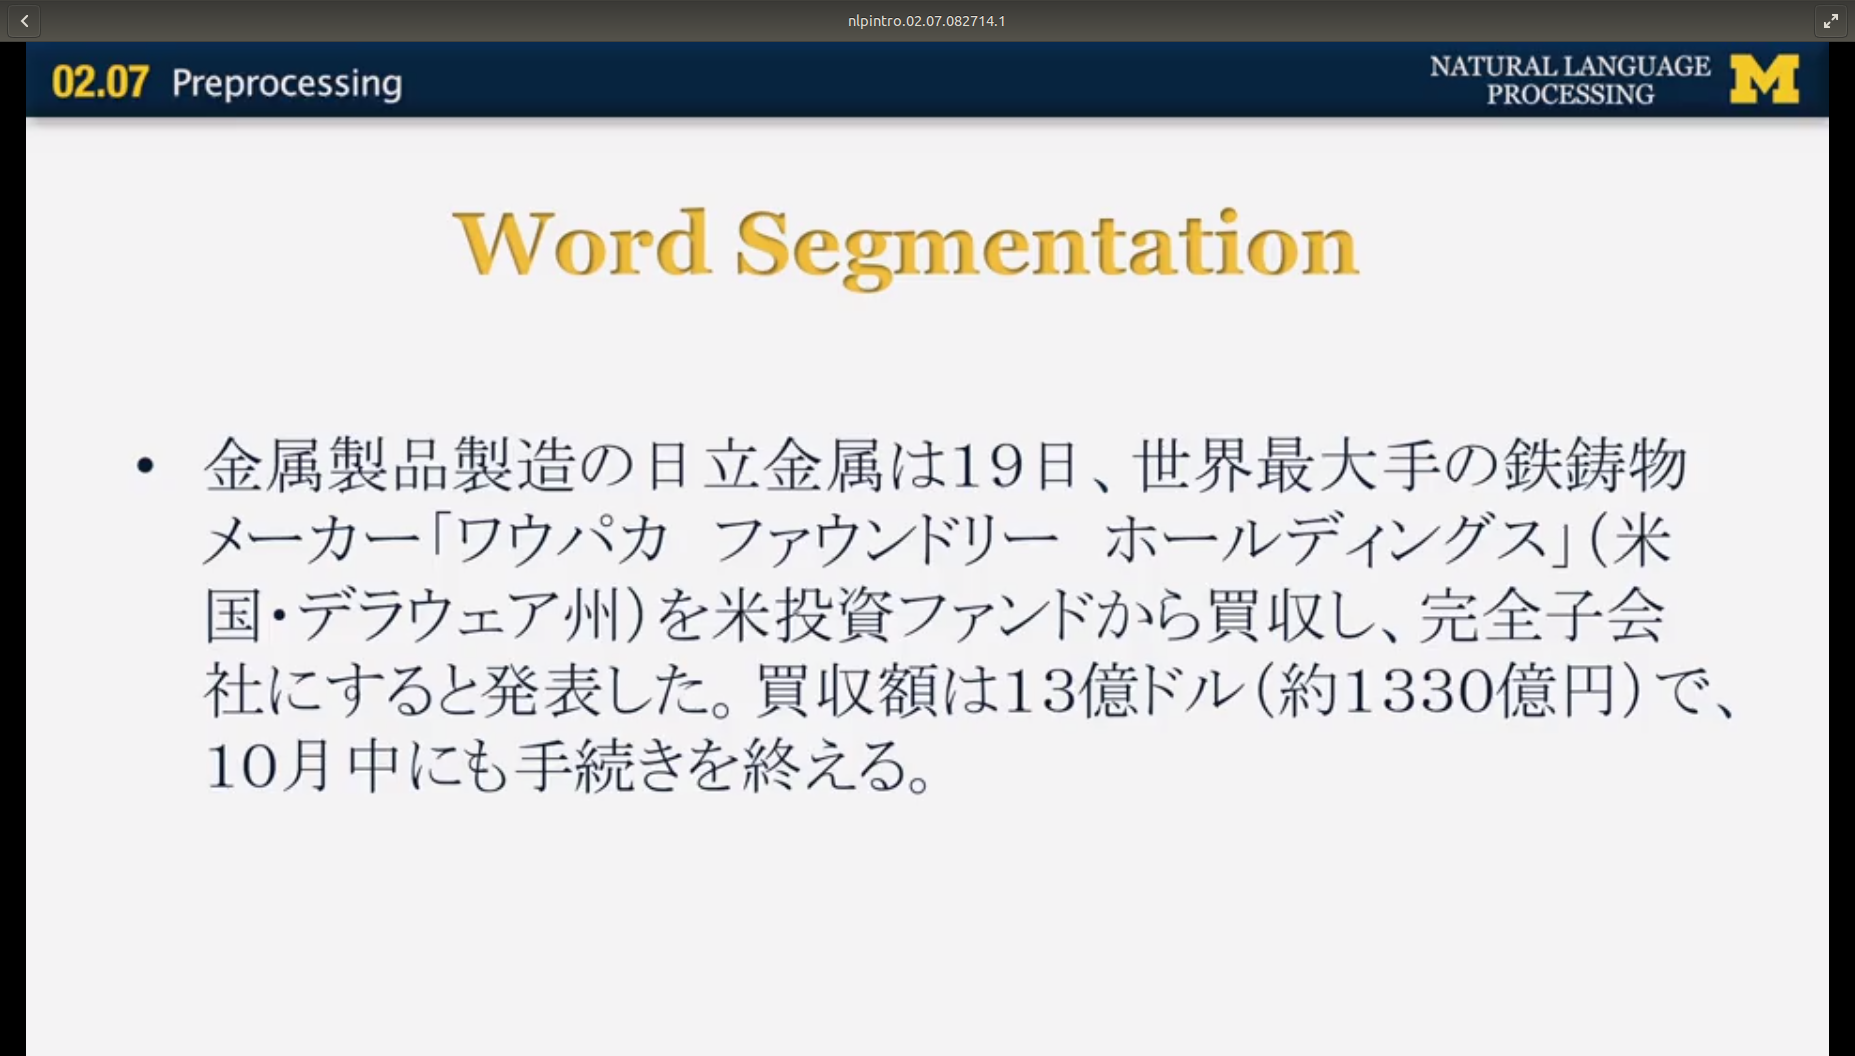
\includegraphics[width=0.9\textwidth]{JapSegmentation-Radev.png}
\end{center}
(Source: Radev's coursera course, Week 2, lecture on pre-processing)
\end{frame}

\begin{frame}
\frametitle{Tokenizing: Conclusion}
Tokenizing is not as easy as it seems. But, a lot of English tokenizing issues can be handled by current day tokenizers (with heavy use of regular expressions). Customized tokenizers for different types of data too exist. For languages such as Japanese and Chinese, there are existing tools (for relatively Standard form of language).
\bigskip Here is an example tokenizer code: \url{http://goo.gl/vJQTAz}

\end{frame}

\begin{frame}
\begin{center}
\Large Text preprocessing: Sentence Splitting
\end{center}
\end{frame}

\begin{frame}
\frametitle{What does sentence splitting do?}
\begin{itemize}
\item Splits the text into sentences. 
\item Sentence splitting is essential to do any higher order NLP task such as parsing, discourse and semantic analysis. 
\item Typically done by writing regular expressions, constructing decision trees of rules, and using machine learning methods (more on this last one later)
\item Issues: Not all sentences end in a full stop. Some have other punctuation markers. Some punctuation can be ambiguous.
\item One code that can learn sentence splitting by itself from large amounts of data: \url{http://www.nltk.org/\_modules/nltk/tokenize/punkt.html}
\end{itemize}
\end{frame}

\begin{frame}
\frametitle{What is the big deal about sentence splitting?}
Just splitting in full-stop or ? or ! will not do.
\begin{itemize}
\item This sentence: "There are several methods such as A, B, C etc., but there is no best method yet. It is a work in progress." 
\item People don't follow conventions or grammar sometimes. Missing capitalization at the start of a sentence, not leaving a space after sentence breaker etc.
\item Spoken language, tweets etc - do not follow same conventions as news articles. This diversity may affect the accuracy of our sentence splitting rules.
\end{itemize}
\end{frame}

\begin{frame}
\frametitle{Sentence splitting conclusion}
While sentence splitting for English in its standard usage is a good, there are some issues with learner texts and other non-canonical forms. Good sentence splitters exist for English like languages. About others: Figure out. 

\bigskip Question: If English did not have capitalization, how easy or difficult would this task be? 
\end{frame}

\begin{frame}
\begin{center}
\Large Practice Exercises
\end{center}
\end{frame}

\begin{frame}
\frametitle{Practice with general Python}
\begin{itemize}
\item Write a tokenizer that splits a sentence into tokens, based on your definition of tokens, and using regular expressions.
\item Write a sentence splitter, that splits a text into sentences, using regular expressions.
\item Test both your tokenizer and sentence splitter by giving some noisy text (tweets, or non-native language, speech transcripts etc.)
\end{itemize}
\end{frame}

\begin{frame}
\frametitle{Practice with NLTK}
\begin{itemize}
\item There are a couple of word tokenizer implementations in NLTK. Explore the differences between the following tokenizers you can access from nltk.tokenize package: TreebankWordTokenizer, StringTokenizer, TweetTokenizer, MWETokenizer, RegExpTokenizer (Take a collection of common sentences and compare how they perform).
\item What is the difference between WordPunktTokenizer and PunktWordTokenizer?
\item Figure out how to do sentence splitting in Python using NLTK, and how many options exist.
\item Finally: If you are interested, explore tokenization/sentence splitting options in NLTK for a non-English language (from documentation)
\end{itemize}
\end{frame}

\begin{frame}
\frametitle{Next Week}
\begin{itemize}
\item Topics: Spelling Errors, Normalization, Morphological analysis
\item Readings: Chapter 2 in J \&M, Chapter 3 in NLTK Book
\item Video lectures: Week 2, and first 2 lectures in Week 3 from Radev's coursera course.
\item Assignment 1 - submit before midnight on saturday
\item I will try to grade before tuesday's class as much as possible.
\end{itemize}
\end{frame}

\end{document}


